\section{Formal Rules and Derivations}
\label{app:proofs}

\subsection{Finite propagation and contribution conservation}
\label{app:conservation}
For an operation $v=f(u_1,\ldots,u_k)$, \dt{} constructs linear maps $D_j$ from the two executions such that
\begin{equation}
\D v=\sum_{j=1}^k D_j\D u_j.
\label{eq:local}
\end{equation}
The incoming slopes $m_v$ propagate to input $j$ as $D_j^\top m_v$. Slopes from multiple consumers add at their shared input. Starting with slope $1$ at the scalar target, the reverse pass produces the source slopes in Equation~\ref{eq:attribution}. For a scalar nonlinearity $f$, the local slope is the divided difference $(f(u_1)-f(u_0))/(u_1-u_0)$, with its derivative as the coincident-input limit. Linear transformations retain their weights, and addition sends the slope to each summand.

\begin{theorem}[Contribution conservation]
For an acyclic computation over real-valued operations satisfying Equation~\ref{eq:local}, reverse propagation from a scalar target yields the conservation identity in Equation~\ref{eq:attribution}.
\end{theorem}
\begin{proof}
An acyclic computation can be expanded into elementary operations with explicit branches. At an operation $v=f(u_1,\ldots,u_k)$, Equation~\ref{eq:local} gives
\begin{equation}
\ip{m_v}{\D v}=\sum_j\ip{D_j^\top m_v}{\D u_j}.
\end{equation}
Replacing a node's contribution by the contributions of its parents therefore preserves the total on a cut through the graph. At shared parents, slopes from different consumers sum. Repeated substitution reaches the input cut and yields Equation~\ref{eq:attribution}, since the slope of the scalar target is $1$. Constant inputs have zero difference and contribute zero to this sum.

\end{proof}

\subsection{Finite attention normalization}
\label{app:softmax}
For an attention row $p_b=\sm(z_b)$, $b\in\{0,1\}$, the finite rule first converts changes in log-probabilities into changes in probabilities. The slope of this conversion is the logarithmic mean $\ell_i$. We define it and its sum as
\begin{equation}
\ell_i=\frac{p_{1,i}-p_{0,i}}{\log p_{1,i}-\log p_{0,i}},\qquad
\tau=\sum_i\ell_i,
\label{eq:logmean}
\end{equation}
with $\ell_i=p_{0,i}$ at coincident probabilities. Dividing by $\tau$ gives weights that sum to one for the row averages below. All quantities are evaluated on the common unmasked support.
\begin{proposition}[Finite attention normalization]
For finite logits on a common support,
\begin{equation}
\D p=\left(\diag(\ell)-\frac{\ell\ell^\top}{\tau}\right)\D z.
\label{eq:softmax}
\end{equation}
\end{proposition}
\begin{proof}
The common support contains positive probabilities. For endpoint $b$, $\log p_b=z_b-a_b\mathbf 1$, where $a_b=\log\sum_i\exp(z_{b,i})$. The definition of the logarithmic mean gives
\begin{equation}
\D p=\ell\odot(\D z-\D a\,\mathbf 1).
\end{equation}
Probability normalization implies $\mathbf 1^\top\D p=0$, so
\begin{equation}
\D a=\frac{\ell^\top\D z}{\tau}.
\end{equation}
Substitution proves Equation~\ref{eq:softmax}. For a target coordinate $y$,
\begin{equation}
\D\log p_y=\left(e_y-\frac{\ell}{\tau}\right)^\top\D z.
\end{equation}
The coincident-probability definition follows from the continuous limit of the logarithmic mean.

\end{proof}
The operator is symmetric. For incoming slopes $m_p$ at probabilities $p$, the slope at query--key score $z_i$ is
\begin{equation}
m_{z,i}=\ell_i(m_{p,i}-\bar m_p),\qquad
\bar m_p=\frac{\sum_j\ell_j m_{p,j}}{\sum_j\ell_j}.
\label{eq:softmax-vjp}
\end{equation}
The slopes for a log-softmax target are $m_z=e_y-\ell/\tau$, where $e_y$ is the one-hot vector selecting the target vocabulary coordinate.

\subsection{Finite operator rules}
\label{app:operators}
For the attention example with output $Y=PV$, Equation~\ref{eq:pv} gives the slopes $m_V=\bar P^\top m_Y$ and $m_P=m_Y\bar V^\top$ for an incoming slope matrix $m_Y$.

Query--key scores use the symmetric product identity,
\begin{equation}
\D(QK^\top)=\D Q\,\bar K^\top+\bar Q\,\D K^\top,\qquad
\bar Q=(Q_0+Q_1)/2,
\label{eq:qk}
\end{equation}
with $\bar K$ defined in the same way. Table~\ref{tab:rules} lists the finite decompositions by operator. Normalization, rotary position transformations, and grouped heads follow their respective model definitions.

\begin{table}[htbp]
\centering
\small
\caption{Finite propagation rules by operator. Bars denote endpoint averages. The gated-memory recurrence is given in Appendix~\ref{app:memory}.}
\label{tab:rules}
\begin{tabular}{@{}p{0.27\linewidth}p{0.65\linewidth}@{}}
\toprule
Operation & Change decomposition \\
\midrule
Linear and residual & $\D(Wx+b)=W\D x$; $\D(a+b)=\D a+\D b$ \\
Attention values & $\D(PV)=\bar P\D V+\D P\bar V$ \\
Attention scores & $\D(QK^\top)=\D Q\bar K^\top+\bar Q\D K^\top$ \\
SwiGLU & $\D(us)=\bar s\odot\D u+\bar u\odot\D s$, $s=\silu(g)$ \\
GDN output gating & $\D(n\odot s)=\bar s\odot\D n+\bar n\odot\D s$ \\
RMS normalization & Analytic finite rule for $wx/\sqrt{\operatorname{mean}(x^2)+\epsilon}$ \\
\bottomrule
\end{tabular}
\end{table}

\subsection{Backward calculation for the Gated DeltaNet example}
\label{app:memory}
With column vectors and a key-by-value state $S_t\in\R^{d_k\times d_v}$, its per-token computation is
\begin{align}
T_t&=\alpha_t S_{t-1}, & r_t&=T_t^\top k_t, \nonumber\\
c_t&=v_t-r_t, & u_t&=\beta_t c_t, \label{eq:gdn}\\
S_t&=T_t+k_tu_t^\top, & o_t&=S_t^\top q_t. \nonumber
\end{align}
The query includes the model's fixed attention scale. $T_t$ is the retained state, $r_t$ is its readout at key $k_t$, and $u_t$ is the gated difference between the incoming value and that readout. One endpoint ordering constructs a finite map $D_{\mathrm{GDN}}^{01}$ for the complete memory recurrence through
\begin{align}
\D T_t&=\alpha_{t,1}\D S_{t-1}+S_{t-1,0}\D\alpha_t, \nonumber\\
\D r_t&=(\D T_t)^\top k_{t,1}+T_{t,0}^\top\D k_t, \nonumber\\
\D u_t&=\beta_{t,1}(\D v_t-\D r_t)+c_{t,0}\D\beta_t, \label{eq:gdn-finite}\\
\D S_t&=\D T_t+k_{t,1}\D u_t^\top+\D k_t\,u_{t,0}^\top, \nonumber\\
\D o_t&=(\D S_t)^\top q_{t,1}+S_{t,0}^\top\D q_t. \nonumber
\end{align}
Swapping the reference and original activations used as local slopes gives $D_{\mathrm{GDN}}^{10}$. Within each GDN layer, we average these memory-recurrence maps and propagate the readout slopes as
\begin{equation}
\bar D_{\mathrm{GDN}}=\frac{D_{\mathrm{GDN}}^{01}+D_{\mathrm{GDN}}^{10}}{2},
\qquad m_{\mathrm{in}}=\bar D_{\mathrm{GDN}}^\top m_o.
\label{eq:gdn-symmetric}
\end{equation}
Here $m_o$ collects the slopes of all readouts $o_t$ in the layer, and $m_{\mathrm{in}}$ collects those returned to the recurrence inputs. Equivalently, apply each transpose map to the same $m_o$ and average the returned slopes. Both maps express the same finite output difference, so their mean preserves it. The recurrence returns slopes for values, keys, queries, and both gates, and propagates state slopes to earlier token positions. Scalar gate nonlinearities and query/key normalization use the surrounding network's finite rules. Output gating uses the symmetric product in Table~\ref{tab:rules}, with $n_t$ the normalized readout and $s_t$ its activated output-gate vector.

\subsection{Product and normalization identities}
For a bilinear map $B$, both
\begin{align}
\D B(a,b)&=B(\D a,\bar b)+B(\bar a,\D b),\\
\D B(a,b)&=B(\D a,b_1)+B(a_0,\D b)
\end{align}
follow by expansion. Equation~\ref{eq:pv} and the SwiGLU rule use the first, symmetric identity. The second identity, with the displayed argument ordering, gives the products in Equation~\ref{eq:gdn-finite}. Its swapped ordering gives the other layer map averaged in Equation~\ref{eq:gdn-symmetric}. Subtraction and state addition are linear.

For RMS normalization $f(x)=w\odot x/r(x)$, $r(x)=\sqrt{\|x\|^2/d+\epsilon}$, the symmetric product rule gives an analytic local map. With $\bar x=(x_0+x_1)/2$, $r_b=r(x_b)$, and $v=w\odot m$, its transpose action is
\begin{equation}
D_f^\top m=
\frac{r_0^{-1}+r_1^{-1}}{2}\,v
-\frac{2\bar x\,\ip{\bar x}{v}}{d\,r_0r_1(r_0+r_1)}.
\end{equation}
The identity follows from $\D r=(2\ip{\bar x}{\D x}/d)/(r_0+r_1)$ and $\D(r^{-1})=-\D r/(r_0r_1)$. The same construction covers fixed learned scale parameters and the query/key normalization used in the memory path.


\section{Implementation and Storage Accounting}
\label{app:computation}

\paragraph{Attention.}
Native endpoint queries, keys, values, and log-normalizers determine the probabilities within each FlashAttention tile. The first sweep accumulates the logarithmic-mean normalizers and weighted row averages in Equation~\ref{eq:softmax-vjp}. Subsequent sweeps accumulate query, key, and value slopes. Endpoint averages reside in linear-size buffers or are computed inside the tiles.

\paragraph{Memory.}
The implementation processes 64-token chunks using FLA's native chunk-state adjoints and batched contractions with saved endpoint states. An associative affine scan computes the finite decay contribution. Convolutions and linear projections propagate slopes through their transpose operations.

\paragraph{Storage.}
For sequence length $T$, head dimension $d$, and tile or chunk width $C$, attention vectors and row statistics occupy $O(Td)$ storage per head. Pairwise products reside in bounded tiles. Dense attention arithmetic is $O(T^2d)$. Chunked memory occupies $O(Td+TC+(T/C)d^2)$ auxiliary storage per head for token slopes, within-chunk products, and boundary states. Both storage expressions are linear in $T$ at fixed $d$ and $C$. Layer replay supplies intermediate activations, with checkpoint storage accounted for separately.

\clearpage
\section{Evaluation Specification}
\label{app:evaluation}
Both models use the released prompts, stored responses, eligible source positions, and evidence annotations. Table~\ref{tab:qwen35-quality} specifies the Qwen3.5 examples for each task. An eligible position is an input position included in the task's attribution and deletion domain. For NIAH, this domain follows the released token selection. VT and HotpotQA recovery select from the passage body.

\paragraph{Baseline comparisons.}
VT and HotpotQA recovery compare all seven methods on the same 448 inputs. The paired development comparison uses the same inputs and stored responses for DT and FT on each model, with one FT recursive step for faithfulness and three for recovery.

\begin{table}[!htb]
\centering\small
\caption{Attribution methods.}
\label{tab:baseline-methods}
\setlength{\tabcolsep}{4pt}
\renewcommand{\arraystretch}{1.15}
\begin{tabular}{@{}>{\raggedright\arraybackslash}p{.17\linewidth}>{\raggedright\arraybackslash}p{.27\linewidth}>{\raggedright\arraybackslash}p{.20\linewidth}>{\raggedright\arraybackslash}p{\dimexpr.36\linewidth-6\tabcolsep\relax}@{}}
\toprule
Method & Principle & Strength & DT advantage \\
\midrule
Perturbation\newline\citep{pan2026flashtrace} & Measure effects of separate masks & Direct intervention & Additive allocation of the joint effect \\
\addlinespace[4pt]
REAGENT\newline\citep{zhao2024reagent} & Iteratively replace tokens and update importance & Black-box attribution & Signed scores without iterative sampling \\
\addlinespace[4pt]
CLP\newline\citep{cifka2023context} & Measure prediction changes as context expands & Reveals newly added information & Allocates the joint effect of selected inputs \\
\addlinespace[4pt]
IFR\newline\citep{ferrando2024information} & Trace contributions to internal representations & Identifies information paths & Includes changes in attention weights \\
\addlinespace[4pt]
AttnLRP\newline\citep{achtibat2024attnlrp} & Propagate output relevance backward & Input and neuron attribution & Explains the measured finite score change \\
\addlinespace[4pt]
FlashTrace\newline\citep{pan2026flashtrace} & Aggregate spans and recursively trace sources & Efficient multi-token attribution & Signed, additive response-score contributions \\
\bottomrule
\end{tabular}
\end{table}

\paragraph{Deletion scores.}
For token attribution scores $A$, DT ranks tokens by $A_i$ for RISE and by $\max(A_i,0)$ for MAS. The evaluator records 21 response scores across 20 deletion steps. Each score sums log-probabilities over the full fixed response plus EOS. Masking all eligible tokens with EOS gives the attribution reference. Full-input and fully-masked scores define the normalization endpoints. The normalized values are clipped to $[0,1]$ and made nonincreasing by a cumulative minimum. For MAS, the remaining attribution share is the positive-score sum over unmasked tokens divided by the initial positive-score sum over eligible tokens. We add its absolute difference from the normalized response score to that score, clip to $[0,1]$, and rescale the resulting curve to $[0,1]$ by its minimum and maximum. MAS is the trapezoidal area under this curve. The case-study curves use the positive ranking and share these endpoints between DT and FT for each model and example.

\paragraph{Recovery targets and budgets.}
For NIAH, DT attributes the full response plus EOS. We select the top 10\% of eligible input tokens ranked by positive-part attribution scores. VT scores the answer tokens and ranks positive body-token scores. Its H2/H4/H6/H10 budgets are 10\%/10\%/20\%/30\%. HotpotQA scores the full response, ranks passage sentences by the sum of their positive token contributions, and selects the longest ranked sentence prefix within 30\% of all body tokens. NIAH/VT report the fraction of annotated evidence tokens recovered. HotpotQA reports Full-support Recall@30\%. Each example scores one if every official supporting fact is selected and zero otherwise. The reported value is the mean across examples.

\begin{table}[htbp]
\centering\small
\caption{Paired development results: the first eight MQ-Q2 and eight MoreHopQA examples per model. These 32 model--example pairs form a separate development set. FT uses one recursive hop for RISE/MAS and three for recovery. RISE is signed; MAS and recovery use positive scores.}
\label{tab:development}
\begin{tabular}{@{}lllrrr@{}}
\toprule
Model & Task & Method & RISE $\downarrow$ & MAS $\downarrow$ & Recovery@10\% $\uparrow$ \\
\midrule
Qwen3-8B & MQ-Q2 & FlashTrace & 0.0685 & 0.1547 & 56.45 \\
 &  & \dt{} & 0.0574 & 0.0806 & 77.52 \\
 & MoreHopQA & FlashTrace & 0.1111 & 0.1969 & --- \\
 &  & \dt{} & 0.0585 & 0.1173 & --- \\
\midrule
Qwen3.5-9B & MQ-Q2 & FlashTrace & 0.0942 & 0.2485 & 63.92 \\
 &  & \dt{} & 0.1115 & 0.1518 & 73.35 \\
 & MoreHopQA & FlashTrace & 0.2356 & 0.2797 & --- \\
 &  & \dt{} & 0.1688 & 0.2426 & --- \\
\bottomrule
\end{tabular}
\end{table}


\section{Implementation Cost Measurements}
\label{app:cost}
DT and one-hop FT use the same inputs and responses in each timing comparison. Time covers the complete attribution call, including returning the source scores. For DT, this includes both forward executions and the reverse pass. Peak allocated device memory includes model weights.

\paragraph{Paired Qwen3 cost.}
Each method has one warm call followed by three measured calls in rotated order on each of 16 development examples. Aggregate times sum the per-example medians.

\paragraph{Response-length comparison.}
The first-page timing panel measures Qwen3-8B on one MetaX C550. Its horizontal axis counts response tokens. Each point is the mean of three complete attribution calls after two warm calls, with a fresh process for each method and length. Error bars show the minimum and maximum measured times.

\clearpage
\section{Detailed Signed Evidence Views}
\begin{figure}[p]
\centering
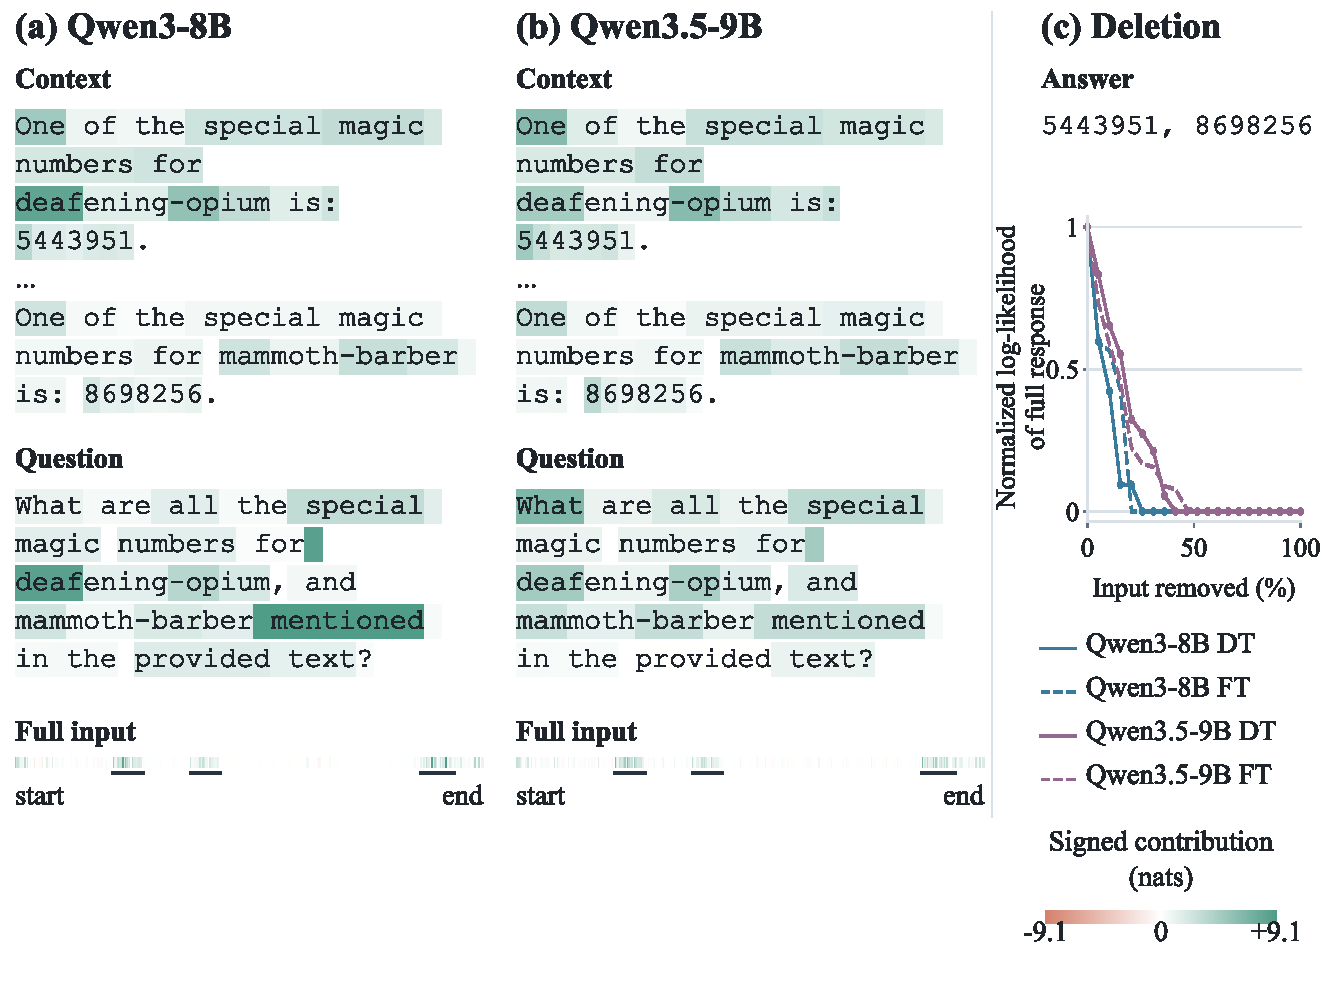
\includegraphics[width=\linewidth]{figures/generated/deltatrace-retrieval.pdf}
\caption{\textbf{Signed evidence for retrieving two numbers.} The first \texttt{niah\_mq\_q2} development example on both models. Token contributions use a shared linear scale in nats: teal raises and coral lowers the score. Underlines locate excerpts in the full input. Attribution targets the complete released response plus EOS; the panel summarizes its answer. Curves show the saved normalized score across 20-step deletion, ranked by positive contribution.}
\label{fig:retrieval}
\end{figure}

\begin{figure}[p]
\centering
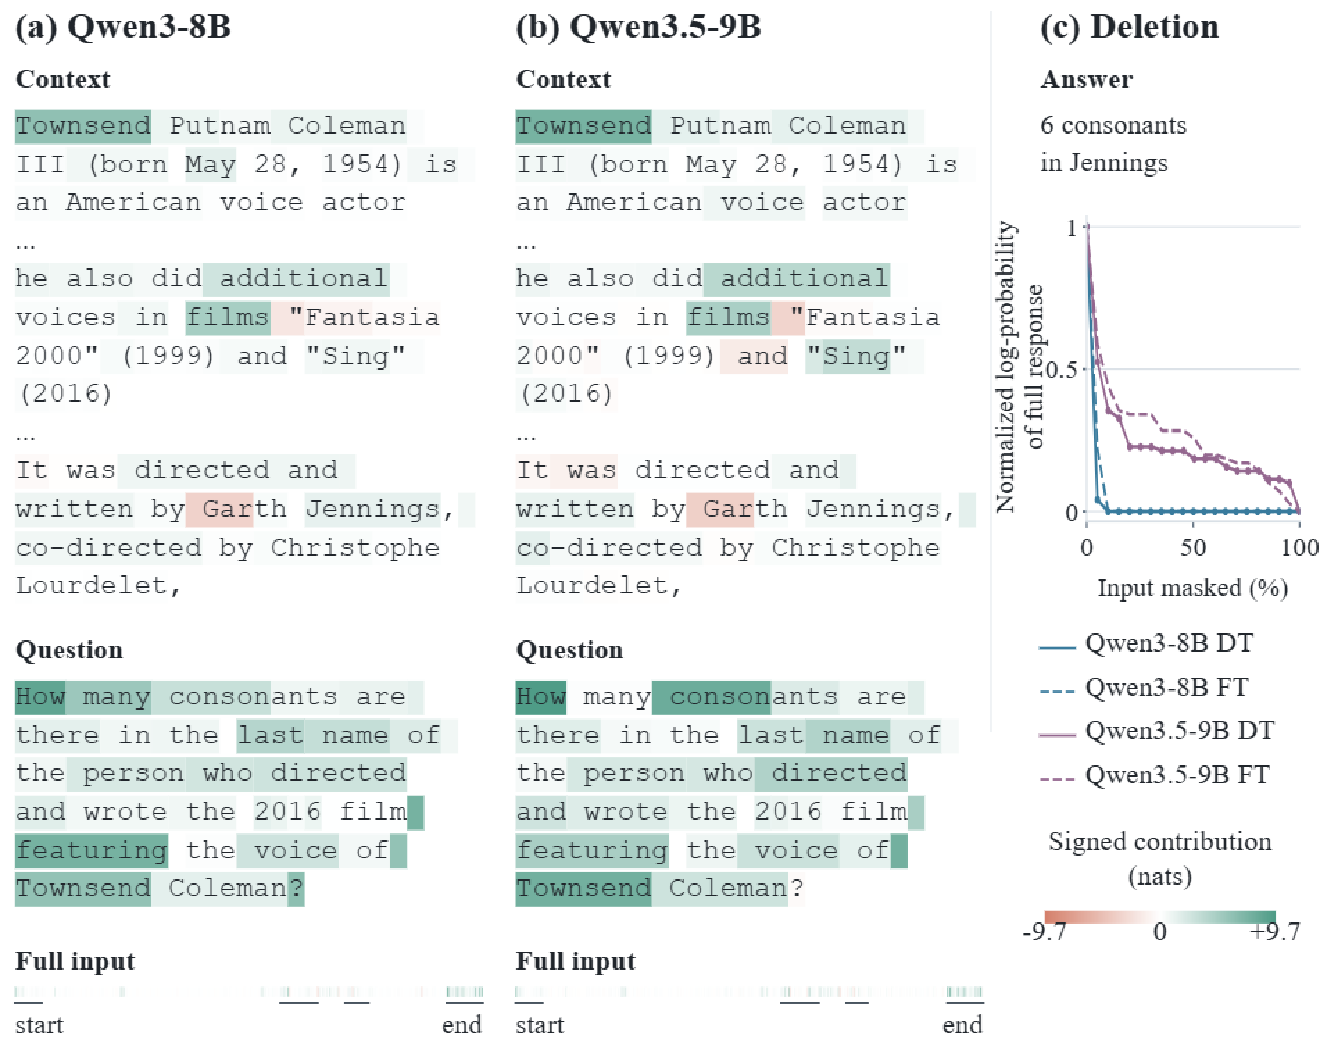
\includegraphics[width=\linewidth]{figures/generated/deltatrace-multihop.pdf}
\caption{\textbf{Signed evidence across a multi-hop question.} The first \texttt{morehopqa} development example links Townsend Coleman to \emph{Sing}, Garth Jennings, and his surname's consonants. Colors, markers, targets, and deletion curves follow Figure~\ref{fig:retrieval}; both models share the scale within this example.}
\label{fig:multihop}
\end{figure}


\clearpage
\section{Counterfactual Credit and Policy Learning}
\label{app:credit}

Under a fixed continuation policy, the expected return difference between an action and a reference action drawn from that policy equals the action's advantage. This identity expresses the action-independent-baseline principle \citep{sutton1999policy} in counterfactual form. COMA uses the related construction to assign credit by averaging one agent's action while fixing the others \citep{foerster2018counterfactual}.

Let $h$ be a decision history and $\pi$ a fixed continuation policy. Write $G^\pi(h,a;\xi)$ for the integrable return obtained by setting the current action to $a$ and subsequently following $\pi$, with $\xi$ supplying environment and policy randomness. Define
\begin{equation}
Q^\pi(h,a)=\mathbb E_\xi[G^\pi(h,a;\xi)],\qquad
V^\pi(h)=\mathbb E_{a'\sim\pi(\cdot\mid h)}[Q^\pi(h,a')].
\end{equation}
The reference action $a'$ is sampled independently of the selected action $a$, conditional on $h$. The two rollouts may share randomness, with each retaining its correct marginal distribution under the corresponding action intervention.

\begin{proposition}[Exactly averaged counterfactual credit]
Under these definitions, the policy-averaged counterfactual credit satisfies
\begin{equation}
C^\pi(h,a)
=\mathbb E_{a',\xi}\!\left[G^\pi(h,a;\xi)-G^\pi(h,a';\xi)\right]
=Q^\pi(h,a)-V^\pi(h).
\label{eq:credit-advantage}
\end{equation}
For a differentiable policy $\pi_\theta$ with positive probabilities over a fixed finite action set, the score-function learning signals obey
\begin{equation}
\mathbb E_{a\sim\pi_\theta}\!\left[\nabla_\theta\log\pi_\theta(a\mid h)\,C^{\pi_\theta}(h,a)\right]
=\mathbb E_{a\sim\pi_\theta}\!\left[\nabla_\theta\log\pi_\theta(a\mid h)\,Q^{\pi_\theta}(h,a)\right].
\label{eq:credit-gradient}
\end{equation}
\end{proposition}
\begin{proof}
Linearity of expectation gives Equation~\ref{eq:credit-advantage}. The baseline term in Equation~\ref{eq:credit-gradient} is
\begin{equation}
V^{\pi_\theta}(h)\sum_a\pi_\theta(a\mid h)\nabla_\theta\log\pi_\theta(a\mid h)
=V^{\pi_\theta}(h)\nabla_\theta\sum_a\pi_\theta(a\mid h)=0.
\end{equation}
Subtracting this term proves the result. Credit and action value serve as weights in the score-function update.
\end{proof}

This equality provides a concrete target for extending finite attribution to learning. The averaged action credit of a reward-level construction should recover the advantage.
